\documentclass[pra,
aps,
twocolumn,
superscriptaddress,
groupedaddress,
nofootinbib,
reprint
]{revtex4-1}

% PACKAGES
\usepackage{amsmath,amsfonts, amssymb, amsthm}
\usepackage{bm, bbm, physics, mathtools}
\usepackage{graphicx, subfigure}
\usepackage{xcolor, enumerate}
\usepackage{xifthen, hyperref}
\usepackage[capitalise]{cleveref}

\hypersetup{
	colorlinks=true,  
	linkcolor=blue,   
	citecolor=blue,   
	urlcolor=blue     
}

\newcommand{\crefrangeconjunction}{--}
\creflabelformat{figure}{(#2#1#3)}

% COMMENT NOTATION
\newcommand{\nick}[1]{{\color{red}#1}}
\newcommand{\ddd}[1]{\textcolor{blue}{#1}}

% ENVIRONMENTS
\newtheorem{theorem}{Theorem}
\newtheorem{proposition}[theorem]{Proposition}
\newtheorem{lemma}[theorem]{Lemma}
\newtheorem{definition}[theorem]{Definition}

% REFERENCES
\iffalse
\renewcommand{\eqref}[1]{Eq.~(\ref{#1})}
\newcommand{\figref}[1]{Fig.~(\ref{#1})}
\newcommand{\tabref}[1]{Tab.~(\ref{#1})}
\newcommand{\secref}[1]{Section~(\ref{#1})}
\newcommand{\appref}[1]{Appendix~(\ref{#1})}
\newcommand{\defref}[1]{Definition~\ref{#1}}
\newcommand{\lemref}[1]{Lemma~\ref{#1}}
\newcommand{\thmref}[1]{Theorem~\ref{#1}}
\fi

% SYMBOL DEFINITIONS
\renewcommand{\cal}[1]{\mathcal{#1}}

\newcommand{\reals}{\mathbb{R}}
\newcommand{\id}{\mathbbm{1}}
\newcommand{\idc}{1_{\rm{C}}}
\newcommand{\supf}{\mathfrak{c}}
\renewcommand{\tr}{{\rm{tr}}}
\renewcommand{\det}{{\rm{det}}}
\newcommand{\floor}[1]{\left\lfloor #1 \right\rfloor}
\newcommand{\ent}[2]{S\left( #1 \middle\vert\middle\vert #2 \right)}
\newcommand{\ents}{{\ent{\frac{m}{n}}{p}}}

\def\dummy{\ell}
\def\NN{n}
\def\mmf{i}
\def\nnf{n}
\def\mlt{m}
\def\ii{i}
\def\jj{j}
\def\kk{k}
\def\II{I}
\def\nn{n}
\def\tt{n'}
\def\mm{a}
\def\wp{u}
\def\wn{v}

\newcommand{\too}[1]{^{\otimes #1}}
\newcommand{\noisys}{\rho_{\rm{S}}}
\newcommand{\noisysn}{\rho_{\rm{S}}(\epsilon)^{\otimes \nn}}
\newcommand{\noisysN}{\rho_{\rm{S}}(\epsilon)^{\otimes \NN}}

\newcommand{\spanv}[1]{
    {{\rm{span}}\left\{#1\right\}}
}
\newcommand{\conv}[1]{
    {{\rm{conv}}#1}
}
\newcommand{\orb}[1]{
    {{\rm{orb}}(#1)}
}
\newcommand{\sn}[1]{
    {{\rm{sn}}\left(#1\right)}
}
\newcommand{\mana}[1]{
    {{\rm{mana}}\left(#1\right)}
}
\newcommand{\lc}[2]{
	{{\rm{L}}_{#1|#2}}
}

\newcommand{\bmx}{\bm{x}}
\newcommand{\bmy}{\bm{y}}
\newcommand{\bmz}{\bm{z}}
\newcommand{\bmu}{\bm{u}}
\newcommand{\bmw}{\bm{w}}
\newcommand{\bmo}{\bm{0}}
\newcommand{\bmd}{\bm{d}}
\newcommand{\bma}{\bm{a}}
\newcommand{\bmxi}{\bm{\xi}}
\newcommand{\bmg}{\bm{g}}

\newcommand{\zd}[1][]{
    \ifthenelse{\isempty{#1}}{
    {\mathbb{Z}_d} }{
    {\mathbb{Z}_{#1}}}
}
\newcommand{\hd}[1][]{
    \ifthenelse{\isempty{#1}}{
    {\cal{H}_d} }{
    {\cal{H}_{#1}}}
}
\newcommand{\pd}[1][]{
    \ifthenelse{\isempty{#1}}{
    {\cal{P}_d} }{
    {\cal{P}_{#1}}}
}
\newcommand{\cd}[1][]{
    \ifthenelse{\isempty{#1}}{
    {\cal{C}_d} }{
    {\cal{C}_{#1}}}
}
\newcommand{\spd}[1][]{
    \ifthenelse{\isempty{#1}}{
    {{\rm{Sp}}(2, \zd)} }{
    {{\rm{Sp}}(2, \zd[#1])}}
}
\newcommand{\gp}[1][]{
    \ifthenelse{\isempty{#1}}{
    {\rm{GP}_d} }{
    {\rm{GP}_{#1}}}
}
\newcommand{\stoch}[1][]{
    \ifthenelse{\isempty{#1}}{
    {{\rm{S}}_d(\bmd)} }{
    {{\rm{S}}_d(#1)}}
}
\newcommand{\stochw}[1][]{
    \ifthenelse{\isempty{#1}}{
    {{\rm{S}}_{d^2}(\W{\sigma})} }{
    {{\rm{S}}_{d^2}(#1)}}
}
\makeatletter
\def\W{\@ifnextchar[{\@with}{\@without}}
\def\@with[#1]#2{ 
    {{\rm{W}}_{#2}\left(#1\right)} }
\def\@without#1{ 
    {{\rm{W}}_{#1}} }
\makeatother

\newcommand{\T}{\cal{T}}
\newcommand{\Z}{\cal{Z}}

\newcommand{\C}{\cal{C}}
\newcommand{\E}{\cal{E}}
\newcommand{\J}{\cal{J}}
\newcommand{\R}{\cal{R}}
\newcommand{\D}{\cal{D}}
\newcommand{\F}{\cal{F}}
\renewcommand{\O}{\cal{O}}
\newcommand{\M}{\cal{M}}

\newcommand{\Fmax}{\F_{\rm{max}}}
\newcommand{\Omax}{\O_{\rm{}max}}
\newcommand{\Rmax}{\R_{\rm{}max}}
\newcommand{\Pis}{\Pi_{\rm{s}}}
\newcommand{\Pio}{\Pi_{\rm{o}}}

\newcommand{\cptp}{{\rm{CPTP}}}
\newcommand{\cpos}{{\rm{CP}}}
\newcommand{\so}{{\rm{SO}}}
\newcommand{\stab}{{\rm{STAB}}}
\newcommand{\spo}{{\rm{SPO}}}
\newcommand{\cspo}{{\rm{CSPO}}}
\newcommand{\rcu}{{\rm{RCU}}}
\newcommand{\tho}{{\rm{TO}}}
\newcommand{\cpwp}{{\rm{CPWPO}}}
\newcommand{\ru}{{\rm{RU}}}


\begin{document}



%%%%%%%%%%%%%%%%%%%%%%%%%%%%%%%%%%%%%%%%
\section{Lower bounds in $\sigma$--fragments}
\ddd{[Am throwing down some rough material, to be polished later.]}

In order to obtain lower bounds one must now make precise what the free operations actually are in the  theory, beyond the condition of preserving Wigner-positivity.

We first consider the unital fragment, and consider the transformations possible using Clifford unitaries, and convex mixtures of Clifford unitaries. We denote the Clifford group as $\C$, and given some quantum state $\rho$ the accessible states in the unital fragment are given by $\E(\rho) = \sum_{g \in \C} p(g) U(g) \rho U(g)^\dagger$.

\subsection{Symplectic majorisation of magic state Wigner distributions.}
We now exploit the the group structure, which leads to a more general notation majorisation that has been extensively studied in the classical context, but to our knowledge has not yet been used in quantum information theory.

\begin{definition} Given a group $G$ that acts on a vector space $V$, we say that $\bmx$ \emph{$G$-majorises} $\bmy$ precisely when $\y \in H(\x)$, where $H(\x)$ is the convex hull of $\{g \x : g \in G\}$. We denote this as $\y \prec_G \x$.
\end{definition}

Now any quantum state $\rho$ has a Wigner distribution $W_\rho(\x)$. Given a Clifford unitary $\U \in \C$ we have that its representation in the Heisenberg-Weyl frame is given by
\begin{equation}
W_{\U(\rho)} (\x) = [\mbox{\ddd{fill in}}].
\end{equation}

This group action corresponds to the action of the affine symplectic group on the discrete phase space $\P_d$. To proceed we can study the discrete translational action, and the symplectic action separately.

\subsection{Cyclic majorisation conditions.}
We can consider for $G$, the cyclic group of order $N$, which is described by $G= \< g | g^N = e\>$. in Terms of the Wigner distributions, this arises for the discrete lattice translations arising from displacement operators.

A set of necessary and sufficient conditions for cyclic majorisation has been obtained and is given as follows. Suppose $\x, \y$ are two real vectors in $\mathbb{R}^n$. Let $\Delta$ be the elementary shift operator, defined by
\begin{equation}
\Delta \x = \Delta (x_1, x_2, \dots, x_n) := (x_n, x_1, x_2, \dots, x_{n-1}),
\end{equation}
and from this it is clear that $\Delta$ generates a representation of the abelian group $(\mathbb{Z}_n,+)$.
We now say that $\x$ \emph{cyclically majorises} $\y$, written $\x \succ_C \y$, if and only if 
\begin{equation}
\y = \sum_{k=0}^{n-1} p_k \Delta^k \x,
\end{equation}
for some probability distribution $p=(p_k)$. This means that $\y$ lies in the convex hull of the orbit of $\x$ under cyclic shifts. Thus, we may write this condition as $\y = L(\p) \x$, where
\begin{equation}
L(\p) :=  \sum_{k=0}^{n-1} p_k \Delta^k,
\end{equation}
is a linear operator, as a function of an unknown distribution $\p$. We now have the following key identity for linear operators of this form:
\begin{equation}
L(\p)\x = QL(\x) \p,
\end{equation}
where $Q$ is a permutation matrix sending $e_0:=(1,0,0,\dots ,0)$ to itself, and otherwise sending $e_k$ to $e_{n-1-k}$, where $e_k=  (0,0,\dots, 0,1,0,\dots, 0)$ is the $k$'th basis vector. We thus have
\begin{align}
\x \succ_C \y &\Leftrightarrow \y = L(\p) \x \mbox{ for some dist. } \p. \nonumber \\
&\Leftrightarrow \y = QL(\x) \p \mbox{ for some dist. } \p. \nonumber \\
&\Leftrightarrow [QL(\x)]^{-1}\y = \p \mbox{ for some dist. } \p. \nonumber \\
&\Leftrightarrow [QL(\x)]^{-1}\y = \p  \ge \mathbf{0} \mbox{ and normalized}.
\end{align}
This implies that to check whether $\x \succ_C \y$ it suffices to compute the components of the left-hand side and ensure non-negativity (I suspect it is normalised if $\x$ and $\y$ are normalised).

Note though that by using Fourier analysis we can simplify this in terms of computational demands to checking if the vector
\begin{equation}
\p = C(\x') Q\y,
\end{equation}
has non-negative components, where
\begin{equation}
\x' := n\F_n [\F_n\x]^{-1},
\end{equation}
with $\F_n$ being the discrete Fourier transform, and the bracket term $[\F_n \x]^{-1}$ denotes the vector obtained by inverting the components of $\F \x$ individually. So the recipe for cyclic majorisation is:
\begin{enumerate}
\item Given inputs $\x$ and $\y$.
\item Compute the vector $\x'$ via two Fourier transforms and $n$ inversions.
\item Compute the circulant matrix $C(\x')$.
\item Compute $\C(\x')Q \y$ and check if all components are non-negative.
\end{enumerate}•


\subsection{Symplectic majorisation for qutrit magic}
The qutrit system provides a good illustration of the techniques. In this case the symplectic group $SL(2,\mathbb{Z}_3)$ is isomorphic (up to $\pm \I$) the symmetry group of the tetrahedron, which in turn is isomorphic to $S_4$, the permutation group on 4 symbols. Therefore we expect in this case that symplectic majorisation on $\P_3$ corresponds to a restricted form of majorisation.


\subsection{Fundamental Regions of a group $G$}
\ddd{[This is theory for the appendices, and also to help flesh out the theory of $G$ majorisation. It looks a bit technical, but the core idea is simple enough once you get it.]}
Given a group $G$ that acts on a vector space $V$, we now have the following concept.
\begin{definition} A \emph{fundamental region} $F$ of $G$ in $V$ is any open set $F$ such that $F \cap gF = \varnothing$ for $g \ne e$ and moreover 
\begin{equation}
V = \bigcup_{g} \overline{g F}.
\end{equation}
\end{definition}
Here, the overline denotes the closure of a set. Loosely speaking, we can view $F$ as obtained by quotienting the vector space $V$ via the group action. We then have the following key theorem, which is proved in [CITE].
\begin{theorem} If $G$ has a fundamental region $F$ that is unique, modulo actions of the group $F\rightarrow gF$, then $\bar{F}$ is a closed, convex cone and for any $\x, \y \in \bar{F}$ we have
\begin{equation}
\y \prec_G \x \Leftrightarrow \mathbf{a}\cdot \y \le \mathbf{a} \cdot \x, \mbox{ for all } \mathbf{a} \in \bar{F}.
\end{equation}
\end{theorem}
If the cone $\bar{F}$ is finitely generated, namely 
\begin{equation}
\bar{F} = \mbox{cone}( \mathbf{c}_1, \dots, \mathbf{c}_N),
\end{equation}
for some finite set of vectors, then the majorisation condition reduces to checking a \emph{finite} set of inequalities, namely checking $\mathbf{c}_k \cdot \y \le \mathbf{c}_k \cdot \x$ for $k=1, \dots , N$.

Note now that any group action $G$ on a vector space $V$ always has a fundamental region. Consider any $\x \in V$ such that $g \x \ne \x$ unless $g =e$. For this we define
\begin{equation}
K = \{ \mathbf{a} \in V : \sup_g \left [ (g\mathbf{a})\cdot \x \right ] = \mathbf{a} \cdot \x \},
\end{equation}
then $F = K_{\mbox{\tiny int}}$ is a fundamental region of $G$ in $V$, where $ K_{\mbox{\tiny int}}$ is the interior of the set $K$. In simple terms, this fundamental region corresponds to the set of vectors that are `close' to $\x$, in the sense that any non-trivial group action $\mathbf{a} \rightarrow g \mathbf{a}$ on them moves them away from $\x$ with respect the inner product. See [CITE] for a proof of this statement.

\subsection{Computing the fundamental region $F$ for the qutrit}
Firstly, note that we actually have that $SL(2, \mathbb{Z}_3)$ is represented by $U(g)$ on $\P_3$, and so we should use that notation for precision.

Since the symplectic group for $d=3$ is a reflection group, it turns out that this guarantees that an essentially unique fundamental region exists, and so we can reduce to a \emph{finite} set of majorisation conditions (I think 5 in this case). Note that the $K$ defined above is always a closed, convex cone. This means it should be `easy' to determine the fundamental region. Reflection groups are Coexter groups, and I believe this set $K$ is essentially a Weyl chamber in that language. Anyhow, let's not get distracted by abstraction.


The concrete recipe going forward:
\begin{enumerate}
\item Pick your favorite $\x \in P_3$ that is \emph{not} stabilized by $g\ne e$. I.e. a vector that moves under all non-trivial group actions.
\item For each $g_k$ look for the extremal cases of $\y$ such that have constant inner product with $\x$. This corresponds to 
\begin{equation}
\left [ (U(g_k) -\I) \y \right ] \cdot \x = 0 \mbox{ for }k=1, \dots ,24.
\end{equation}
Or equivalently,
\begin{equation}
\y \cdot A^T\x = 0,
\end{equation}
where $A := U(g_k) -\I$.
\item Write down the matrix equation for each $g_k$.
\item Each of these conditions defines a hyperplane $H_k$ in $\P_3$ corresponding to the boundary of $K$.
\item We possibly don't need to range over all 24 group elements....but am not sure on this.
\item From this, we should be able to extract a generating set of vectors.
\end{enumerate}

\subsection{Toy example to see how the algorithm works}
Okay, let's see how it works in a simple case. Let's consider the case of $V= \mathbb{R}^2$ and $G=S_2=\<g|g^2=e\>$ with the group action $g.(x,y) = (y,x)$ that swaps the components of the vector. We should get standard majorisation out of this $G$--majorisation.

First we find an $\x$ that transforms non-trivially under non-trivial group actions. The vector $\x=(1,0)$ does this. To construct a fundamental region we now look at the equation 
\begin{equation}
[g.(x,y) - (x,y)] \cdot (1,0) = 0
\end{equation}
and solve for $x,y$. This becomes,
\begin{equation}
(y-x, x-y)\cdot(1,0)=0,
\end{equation}
which implies the hyperplane (line!) $y=x$ is the \emph{boundary} of the fundamental region. Since we decided to start with $(1,0)$ we can take the region to the right of this line, and so:
\begin{equation}
F = \{(x,y) : x>y \}
\end{equation}
where we note that we use the strict inequality to get the interior. The region $\bar{F}$ is a half-space, but this is actually a cone, and can be written as
\begin{equation}
F= \mbox{cone}( (1,1),(-1,-1), (5,0)).
\end{equation}
The first two vectors give the boundary, and we just need one other vector inside $F$ to generate it fully, chosen arbitrarily to be $(5,0)$. This last one is needed since $(1,1)$ and $(-1,-1)$ are linearly dependent! Therefore
\begin{align}
\mathbf{c}_1 &= (1,1) \nonumber \\
\mathbf{c}_2 &= (-1,-1) \nonumber \\
\mathbf{c}_3 &= (5,0).
\end{align}
The $S_2$--majorisation ordering is then given by
\begin{equation}
\y \prec \x \Leftrightarrow \mathbf{c}_k \cdot \y \le  \mathbf{c}_k \cdot \x,
\end{equation}
for $k=1,2,3$ whenever $\x,\y \in F$. Note that is gives the ordering for all vectors in the space, since any general vector can be transformed into $F$ via a group action, since $F$ is a fundamental region. Indeed mapping an $\x$ into $F$ is simply $\x \rightarrow \x^\downarrow$, the sorting maneuver!
The generating vectors $(1,1)$ and $(-1,-1)$ imply that both 
\begin{equation}
y_1 + y_2 \le x_1 +x_2,
\end{equation}
and
\begin{equation}
y_1 + y_2 \ge x_1 +x_2,
\end{equation}
which becomes the majorisation condition
\begin{equation}
y_1+y_2 = x_1 + x_2.
\end{equation}
Easy! The final condition from $\mathbf{c}_3=(1,0)$ is then the condition that
\begin{equation}
5y_1 \le 5x_1 \Rightarrow y_1 \le x_1,
\end{equation}
which is the final majorisation condition. Thus we have shown how the familiar majorisation structure corresponds to the theory of $G$--majorisation, and the cone ordering structure that comes from fundamental regions.

\subsection{Another toy example -- non-standard majorisation this time}
Okay, let's look at another option for $V=\mathbb{R}^2$. Now consider the group $G=\mathbb{Z}_2 \times \mathbb{Z}_2$ that can be represented as $G=\<g_1,g_2 | g^1=e, g_2 = e, g_1g_2 = g_2g_1\>$, and acts on vectors as $g_1.(x,y) = (-x,y), g_2.(x,y)=(x,-y)$. In other words the group just flips vectors about X/Y axes.

A vector that moves under the non-trivial group actions is $(1,1)$, so we use this one and solve for $[g.(x,y) - (x,y)] \cdot (1,1) = 0$. We have for $g = g_1$ the equation
\begin{equation}
[(-x,y) - (x,y)]\cdot (1,1) = 0,
\end{equation}
which implies the line $x=0$.

For $g=g_2$ we have
\begin{equation}
[(x,-y) - (x,y)]\cdot (1,1) = 0,
\end{equation}
which implies the line $y=0$.

For $g=g_1g_2$ we have
\begin{equation}
[(-x,-y) - (x,y)]\cdot (1,1) = 0,
\end{equation}
which implies the line $x+y=0$. The open region bounded by these three conditions is the set
\begin{equation}
F := \{ (x,y) : x>0, y>0\}.
\end{equation}
So the positive quadrant of $\mathbb{R}^2$ is a fundamental region for $G$, which makes sense since via sign flips we can map this onto the whole plane, once we close the set. This is again a convex cone and $\bar{F} = \mbox{cone}((1,0), (0,1))$. Thus given any two vectors $\x,\y$ we first act with $G$ to flip their signs so that their components are all positive, $\x \rightarrow \x^\star\ge \mathbf{0}$, then $\y \prec_G \x$ if and only if $y_1 \le x_1$ and $y_2 \le x_2$. This implies that 
\begin{equation}
\y \prec_G \x \Leftrightarrow \y^\star \le \x^\star. 
\end{equation}
So the $G=\mathbb{Z}_2 \times \mathbb{Z}_2$ majorisation gives the component-wise ordering on vectors once you sort them. It is clear that this extends to any $G=\mathbb{Z}_2^{\times n}$.
\subsection{A more complex example $S_3$ on $\mathbb{R}^3$.}
So the symmetric group $S_n$ always gives majorisation. But the symmetric group has $|S_n| = n!$ elements to it, which is super-exponentially big in $n$. We clearly don't have to check $n!$ equations, since the majorisation conditions involve just $n+1$ inequalities, and so it must be that the basic generating conditions of the group suffice to determine the fundamental region of $G$.

Let's look at $V = \mathbb{R}^3$ and $G=S_3$ acting on $\x = (x_i)$ as $g.\x = (x_{g^{-1}}(i))$. A vector that transforms non-trivially under all non-trivial actions is $(2,1,0)$. Let's look at the transpositions, and the boundary planes they give first.

For $g= (1\,\,2)$ we have the equation
\begin{equation}
[(y,x,z) - (x,y,z)] \cdot (2,1,0) = 0,
\end{equation}
which implies the plane $2(y-x)+ x-y = 0$, namely,
\begin{equation}
H_1 = \{(x,y,z) : y=x\}.
\end{equation}
The other choices of transpositions work the same and give the planes
\begin{align}
H_2 &= \{(x,y,z) : y=z\} \\
H_3 &= \{(x,y,z) : x=z\}.
\end{align}
Note that their intersection gives the line $\{(x,y,z) : x=y=z\}$, which is the line of uniform vectors at the bottom of the majorisation pre-order.

What information do the $3$-cycles give? Okay, let's now look at $g=( 1 \,\, 2 \,\, 3)$. The core equation for this becomes
\begin{equation}
[(z,x,y) - (x,y,z)] \cdot (2,1,0) = 0,
\end{equation}
and so gives
\begin{align}
2(z-x) + (x-y) &= 0 \nonumber \\
\Rightarrow x+y &=2z. 
\end{align}
Namely the plane
\begin{equation}
H_4 = \{(x,y,z) :  x+y =2z\}.
\end{equation}The remaining $3$--cycle $(3\,\,2\,\,1)$ gives
\begin{align}
H_5 &= \{(x,y,z) : y+z = 2x\}.
\end{align}
Note that $|S_3| = 6$, but the identity element $g=e$ gives no constraint, and so there are exactly $5$ bounding planes. Note also that the line $\{ (t,t,t)\} $ is again the intersection of all the planes.

These 5 planes bound a cone containing $(2,1,0)$, namely the fundamental region $F$. What's a good algorithm to obtain a generating set of vectors for this cone?

Firstly, since the line $\{(t,t,t)\}$ being the intersection of all the planes, is definitely on the boundary of $F$, this means we must have $\mathbf{c}_1 = (1,1,1)$ and $\mathbf{c}_2 = (-1,-1,-1)$ in our generating set. Perhaps a good algorithm is to compute intersections, obtain generating vectors for these intersections of the hyperplanes, $H_{ij}$ and then let $K_i$ and $K_j$ be the half-spaces in which $(2,1,0)$ resides. Now the intersection of two cones, is itself a cone so we can just keep intersecting the half-space/cones. Thus, we compute
\begin{align}
H_{12} &:= H_1 \cap H_2 \\
&=\{ (t,t,t) : t\in \mathbb{R}\}=:L.
\end{align}
Similarly, $H_{13} = H_{23}= L$. What about the other intersections? Well $H_{14} = H_{15}=L$. In fact all intersections are the same! 
\begin{equation}
H_{ij} = H_i \cap H_j = L \mbox{ for all } i,j.
\end{equation}
The fundamental region is given by the intersection of $K_1$ and $K_2$, or any other two half-spaces. This is generated by $\mathbf{c}_1$ and $\mathbf{c}_2$ above, and any two independent vectors in the intersection of these half-spaces. We can choose 
\begin{align}
\mathbf{c}_3 &= (1,1,0) \\
\mathbf{c}_4 &= (1,0,0),
\end{align}
note that $\mathbf{c}_3 \in H_1$ and $\mathbf{c}_4 \in H_2$, while $\mathbf{c}_3 \in K_2$ and $\mathbf{c}_4 \in K_1$ and so this works correctly. We thus have
\begin{equation}
\bar{F} = \mbox{cone}(\mathbf{c}_1 ,\mathbf{c}_2 ,\mathbf{c}_3 ,\mathbf{c}_4 ).
\end{equation}
The first two inequalities give the condition that
\begin{equation}
x_1+x_2+x_3 = y_1+y_2+y_3,
\end{equation}
while the remaining two conditions give the inequalities
\begin{align}
y_1 &\le x_1 \\
y_1+y_2 &\le x_1 +x_2.
\end{align}
This is the standard majorisation relation. Geometrically, the cone $\bar{F}$ is actually a funny one to visualise: it consists of a half-line radiating out from $(0,0,0)$ to $(-1, -1, -1)$, together with the triangular ``infinite pyramid'' generated by positive combinations of $(1,1,1), (1,1,0), (1,0,0)$. But we can also take positive linear combinations of $(-1,-1,-1)$ and e.g. $(1,1,0)$ and so it is still a bit tricky to visualise.
\subsection{Symplectic majorisation for $d =5$ and beyond.}
For the case $d=5$ we also have a particularly simple group structure, where now the symplectic group $SL(2, \mathbb{Z}_5)$ is isomorphic to the symmetry group of the icosahedron. This is another reflection group and therefore we can again obtain the finite set of majorisation conditions to describe it. Here the order of the group is $60$ and so we probably shouldn't make Nick compute this by hand.

%%%%%%%%%%%%%%%%%%%%%%%%%%%%%%%%%%%%%%%%

\section{Extension to general quantum resource theories}
\label{sec:frag}

So far we have introduced the notion of $\sigma$--fragments for any resource theory of magic. 
In this section we pause to generalise this concept to an arbitrary resource theory and explain precisely how it connects with resource monotones. 
The busy reader more focussed on magic may skip this section.

State convertibility within a given resource theory is often a hard question to address due to the intricate structure of the theory.
In general, the structure of a theory $\R$ is described by a pre-order $\prec_\R$ and usually resource monotones are employed to reduce this structure into a simple real number ordering \nick{CITE}.
The subdivisions of magic theories into $\sigma$--fragments suggests a new approach towards investigating state convertibility which retains more structure of the originaltheory than a measure can.

Monotones reduce the structure of the resource theory $\R$ to a \emph{total} order on the real numbers.
Therefore, two states, even if incomparable in $\R$, are always mapped onto ordered real numbers.
We now generalise this idea of a theory projection that preserves comparability between states. 
\begin{definition}[\textbf{Covariant projection}]\label{def:covproj}
Let $\R = (\F, \O)$ be a resource theory with pre-order $\prec_\R$. 
Then a \emph{covariant resource projection} of $\R$ to a resource theory $\R'$ with pre-order $\prec_{\R'}$, is a pair of mappings $(\Pi_s, \Pi_o)$, where $\Pi_s$ maps quantum states in $\R$ to quantum states in $\R'$, and $\Pi_o$ maps free operations in $\R$ to free operations in $\R'$. 
Moreover, these obey
	\begin{enumerate}
        \item $\Pis(\rho_1) \prec_{\R'} \Pis(\rho_2)$ whenever $\rho_1 \prec_\R \rho_2$;
        \item $\Pio(\E) = \Pio(\E_1) \circ \Pio(\E_2)$ whenever $\E = \E_1 \circ \E_2$.
    \end{enumerate}
We call $\R'$ a \emph{covariant fragment} of $\R$.
\end{definition}

Resource monotones can now be clearly seen as a special case of covariant resource projections.
\begin{proposition}[\textbf{Totally ordered covariant theories}]\label{thm:monoproj}
	Any resource monotone $\M$ of a resource theory $\R$ is a covariant projection for which $\prec_{\R'}$ is a total order. 
	Conversely, any such covariant projection corresponds to a resource monotone $\M$. 
\end{proposition}
\begin{proof}
	Consider a monotone $\M$ in the context of a general resource theory $\R = (\F, \O)$.
	State order is covariantly preserved due to the defining property of a monotone, stated in~\cref{def:mono}, where the pre-order $\prec_{\R'}$ is simply the total order $\leq$ on $\mathbb{R}$. 
	
	Operational composition is covariantly preserved when we simply choose $\Pio(\E) = 1_\times$, namely the `multiplication by 1' operation on real numbers. 
	The definition of a resource monotone then automatically implies covariance.
	
	Conversely, given any covariant projection of $\R$ for which $\prec_{\R'}$ is a total order, we may map the totally ordered set of elements $\Pis(\rho)$ via an injective, non-decreasing function $f$ into $\mathbb{R}$. 
	Then, $\M(\rho):=f(\Pi_s(\rho))$ provides a numerical value for each $\rho$ that obeys the definition of a monotone.
	
\end{proof}

We can also view $\sigma$--fragments as an example of reducing the structure of a magic theory $\R$ to a subtheory with a tractable pre-order.
However, states which are incomparable in $\R$ remain incomparable and conversions between states which are comparable in $\R$ may no longer be possible.
\begin{definition}[\textbf{Contravariant projection}]\label{def:contraproj}
	Let $\R = (\F, \O)$ be a resource theory with pre-order $\prec_\R$. 
Then a \emph{contravariant resource projection} of $\R$ onto a resource theory $\R'$ with pre-order $\prec_{\R'}$, is a pair of mappings $(\Pi_s, \Pi_o)$, where $\Pi_s$ maps quantum states in $\R$ onto quantum states in $\R'$, and $\Pi_o$ maps free operations in $\R$ onto free operations in $\R'$. 
Moreover, these obey
	\begin{enumerate}
        \item $\rho_1 \prec_\R \rho_2$ whenever $\Pis(\rho_1) \prec_{\R'} \Pis(\rho_2)$;
        \item $\E = \E_1 \circ \E_2$ whenever $\Pio(\E) = \Pio(\E_1) \circ \Pio(\E_2)$.
    \end{enumerate}
We call $\R'$ a \emph{contravariant fragment} of $\R$.
\end{definition}
The use of covariant and contravariant in~\cref{def:covproj,def:contraproj} refers to the direction of implication between the two pre-orders and operation compositions\footnote{Note that strictly these are not projections in the sense of $\Pi^2 = \Pi$, but are instead morphisms. 
Here our use of the term projection is motivated by the idea that one one generally loses information about $\R$ under the mapping.}.

\nick{Perhaps scrap definition of contravariant projection and define contravariant fragment as a subtheory $\R'$ where there exists a (injective) covariant projection from $\R'$ to parent theory $\R$. That would make every subtheory $\R' = (\F', \O')$ a contravariant fragment if $\O'$ is closed under composition, this includes $\sigma$--fragments.}

\begin{proposition}\label{thm:subproj}
    Let $\R = (\F, \O)$ be a resource theory, and let $\O' \subseteq \O$ be a non-empty subset of the free operations that is closed under composition, and moreover $\O'$ is the largest such subset, in the sense that for any $\E_1 \not \in \O'$ and any $\E_2 \in \O'$ we have that both $\E_1 \circ \E_2$ and $\E_2 \circ \E_1$ are not in $\O'$. Then $\R' = (\F, \O')$ of $\R$ defines a contravariant fragment of $\R$.    
\end{proposition}
\begin{proof}
    We first define $\Pis (\rho) = \rho$ for all $\rho$. It is clear that since $\O'$ is a subset of $\O$ any operation in $\O'$ will map the set of free states into itself. Moreover the identity channel $id$ is necessarily in $\O'$, due to the maximality assumption. For $\Pio$ we let $\Pis(\E) = \E$ if $\E \in \O'$ and otherwise $\Pis(\E) =id$. Now consider $\Pio (\E_1 \circ \E_2)$. Either the triple $\{\E_1, \E_2, \E_1\circ \E_2\}$ are all in $\O'$ or they are all outside of $\O'$. For the former case $\Pio(\E_1 \circ \E_2) = \E_1 \circ \E_2 = \Pio(\E_1) \circ \Pio(\E_2)$, while for the latter $\Pio(\E_1 \circ \E_2) = id = \Pio(\E_1) \circ \Pio(\E_2)$, which proves that compositions are respected under the map. Finally, $\rho \prec_{R'} \sigma$ implies there exists $\E \in \O' \subseteq \O$ such that $ \E(\rho) = \sigma$, and since $\E \in \O$ this implies $\rho \prec _{\R} \sigma$, as required, which completes the proof.
    
\end{proof}
\nick{Suppose $\E_2$ is the replacement channel $\E_2(\rho) = \sigma$. This is a stabiliser operation. Then $\E_2 \circ \E_1 \in \O_\sigma$ even if $\E_1 \notin \O_\sigma$. Now suppose $\E$ is a Hadamard unitary, then $id = \E \circ \E_{reverse}$ but $id \in \O_{\ketbra{0}}$ while $\E, \E_{reverse} \notin \O_{\ketbra{0}}$.} \ddd{[Ah ok, agreed. This is fine for now. Let's not spend ages trying to generalise this so as to include the majorisation fragments. It's just good to explore the possibilities a bit, to illustrate the non-trivial aspects.]}
As an immediate corollary of~\cref{thm:subproj}, a $\sigma$--fragment of any magic theory $\R$ is a contravariant fragment of $\R$.


\begin{proposition}
	Let $\R = (\F,\O)$ be a resource theory, and let $\D \in \O$ be a free operation, which is reversible by $\D_{\rm{rev}} \in \O$, so that $\D_{\rm{rev}} \circ \D = \idc$.
	
	Then, we can define a contravariant projection of $\R$, by acting on all quantum states with $\D$.
\end{proposition}
\begin{proof}
	We show that the theory $\R' = (\F', \O)$, with $\F' = \{\D(\rho):\rho \in \F \}$, is a contravariant fragment of $\R$.
	
	Let $\Pis$ map every state $\rho$ to $\D(\rho)$ and suppose $\D(\rho_1) \prec \D(\rho_2)$. 
	Then, there exists $\E \in \O$ such that $\rho_1 = (\D_{\rm{rev}} \circ \E \circ \D) (\rho_2)$, so $\rho_1 \prec \rho_2$.
	
	Finally, let $\Pio$ map every free operation to itself, so that composition of operations is trivially preserved.
	
\nick{If $\D$ is a recovery map, so that $\D \circ \D_{\rm{rev}} = \idc$, then this is a covariant projection instead.

If $\D$ is not reversible, this mapping is in general NOT contravariant (consider the replacement map $\D(\rho) = \frac{1}{d}\id$ for a strange state and stabiliser state - surely there is such a counterexample in thermodynamics theory if we consider a highly coherent state and one with the same energy population but no coherences.} \ddd{[Ok. Again, let's not spend time worrying about this now. It's clear there is various fine-print to these cases...but they're not essential to our work so let's put this on hold.]}
\end{proof}

Important examples of resource fragments appear in several established resource theories. \nick{Need to check if the thermodynamics example works, include magic theories as fragments of $\Rmax$, include Nielsen's bipartite entanglement.} \ddd{[Don't worry about these things now -- let's get the computations section improved]}

%%%%%%%%%%%%%%%%%%%%%%%%%%%%%%%%%%%%%%%%

\section{Bound comparison}
An $n$-copy state $\rho^n$ has \emph{error rate} $\delta$ iff $\rho$ has an overlap of at least $1-\delta$ with magic state $\ket{\rm{S}}$,
\begin{equation}
	\bra{\rm{S}}\rho\ket{\rm{S}} \geq 1-\delta.
\end{equation}
The $\epsilon$-noisy Strange state $\rho_{\rm{S}}(\epsilon)^{\otimes n}$ has error rate $\delta = \frac{2}{3}\epsilon$.
A general state of $n$ qutrits with error rate $\delta$ can be converted to the form $\rho_{\rm{S}}(\epsilon_0)^{\otimes n}$ for some noise level $\epsilon$ not necessarily equal to $\delta$.

Given an $[[m,k,d]]$ error correcting code, a distillation protocol that achieves the process in~\cref{eq:test} requires that the following bound holds,
\begin{align}
	\frac{n}{n'} = O(\log^\gamma{(1/\epsilon')}),\ \gamma = \log_d{\left(\frac{m}{k}\right)}
\end{align}

In~\cite{Bravyi2012,Hastings2018}, the asymptotic rate $O(\log^\gamma{(1/\epsilon')})$ is called the \emph{distillation cost}, and in~\cite{cit:bravyi,Krishna2019} the parameter $\gamma$ is called the \emph{overhead}.

There are many distillation protocols in the literature, e.g.~\cite{Bravyi2012,Hastings2018}, that involve a specific value of $\gamma$ and convert a specific number of copies $n$ of input states to $n'=1$ output state \nick{what about $\epsilon$?}.
They should all satisfy
\begin{equation}\label{eq:rate_cost}
	\frac{1}{R(\epsilon, \epsilon', \beta)} \leq \frac{n}{n'} = O(\log^\gamma{(1/\epsilon')}).
\end{equation}
Therefore, given process parameters $n, n', \epsilon, \epsilon'$, we can scan through the stabiliser states to find a range of $\beta$ for which inequality~\cref{eq:rate_cost} is valid.
In principle, the higher the value of parameter $\gamma$, the lower the output error rate $\epsilon'$ can be while~\cref{eq:rate_cost} is still true.
In~\cite{Hastings2018} \nick{CITE MORE}, they report a value of $\gamma = 0.6779\dots$, while in~\cite{Krishna2019}, they report a scaling $\gamma = O(1/\log{d})$ with respect to the system's odd prime dimension $d$.
The latter tends to 0 asymptotically.

We can rephrase this result, saying that any distillation protocol in the $\gamma_\beta$-fragment with an $n$-copy input and $n'$-copy, $\epsilon'$-noisy desired output, must have input noise level 
\begin{equation}
	\epsilon \leq  E\left(\frac{n'}{n}, \epsilon', \beta \right)
\end{equation}
for some error bound $E$ related to $R$.

Furthermore, in~\cite{cit:bravyi,cit:prakash}, two different distillation protocols are proposed with output error rate scalings of the form 
\begin{equation}
	\epsilon' \propto (\alpha \epsilon)^{n^\xi},
\end{equation}
where $\alpha$ is some constant, $\xi = 1/\log_3{15} \approx 0.4$ in~\cite{cit:bravyi} for qubit codes and $\xi = 1/\log_3{19008} \approx 0.1$ for qutrit codes.
They also report a certain input threshold error rate $\epsilon_\star$ above which distillation is not possible.
A first requirement is that $\epsilon_\star \leq E(n'/n, \epsilon', \beta)$, but we can also again find a range of $\beta$ for which the inequality
\begin{align}
	\epsilon &\leq E\left(\frac{n'}{n}, \epsilon'(\epsilon), \beta \right) \\
	\epsilon' &\sim O\left((n\epsilon)^d\right)
\end{align}
holds, given some distillation rate $n'/n$ and input error rate $\epsilon$.


%%%%%%%%%%%%%%%%%%%%%%%%%%%%%%%%%%%%%%%%

\section{Random info}
\begin{figure}[h]
    \centering
    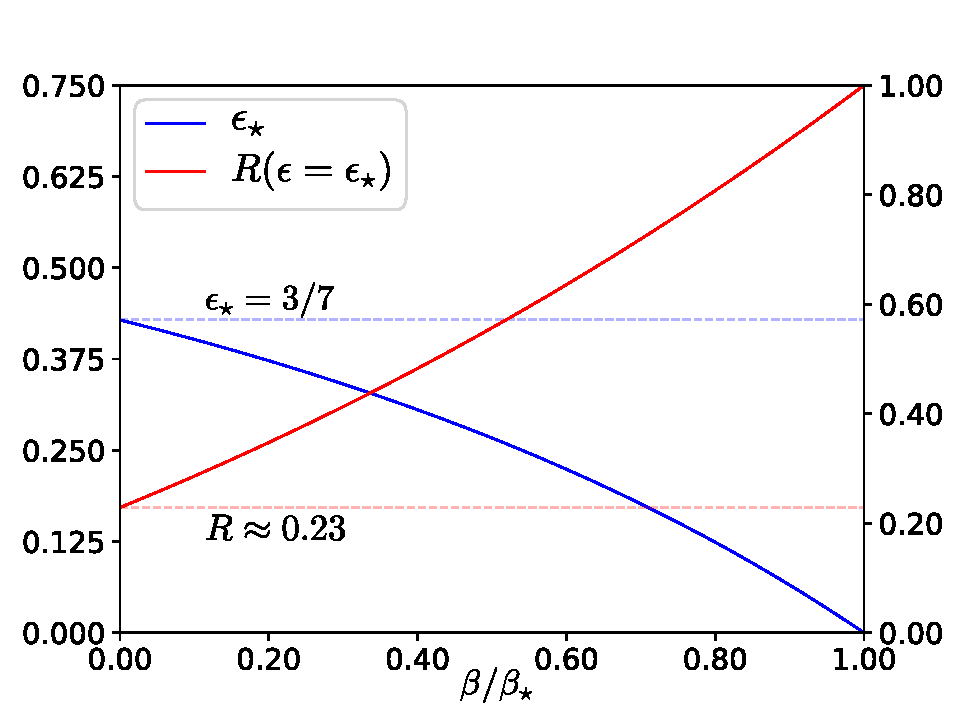
\includegraphics[scale=0.5]{figs/noise_threshold.pdf}
    \caption{\textbf{Noise threshold $\epsilon_\star$ and rate $R(\beta, \epsilon_\star)$ versus $\beta$.}
    At $\beta = 0$ and threshold noise level $\epsilon = \epsilon_\star = 3/7$, the rate is $R(0, \epsilon_\star) = \frac{\ln{(9/7)}}{\ln{3}} \approx 0.23$.
    }
    \label{fig:noise_threshold}
\end{figure}

We generalise the analysis of unital fragments into any circuit with thermalisation noise parametrised by the temperature $\beta^{-1}$.
In~\cref{fig:thermal_distill}, we examine the majorisation bound for the same purification process of~\cref{eq:sdist} with $\epsilon' = 0.05$.
The curves plotted suggest that there exists a fragment $\O_{\gamma_{\beta_{\rm{max}}}}$ which allows for a highest noise threshold at any given number of copies of the initial state.
Adding more copies results in a lower optimal temperature $\beta^{-1}$.

\begin{figure}[h]
    \centering
    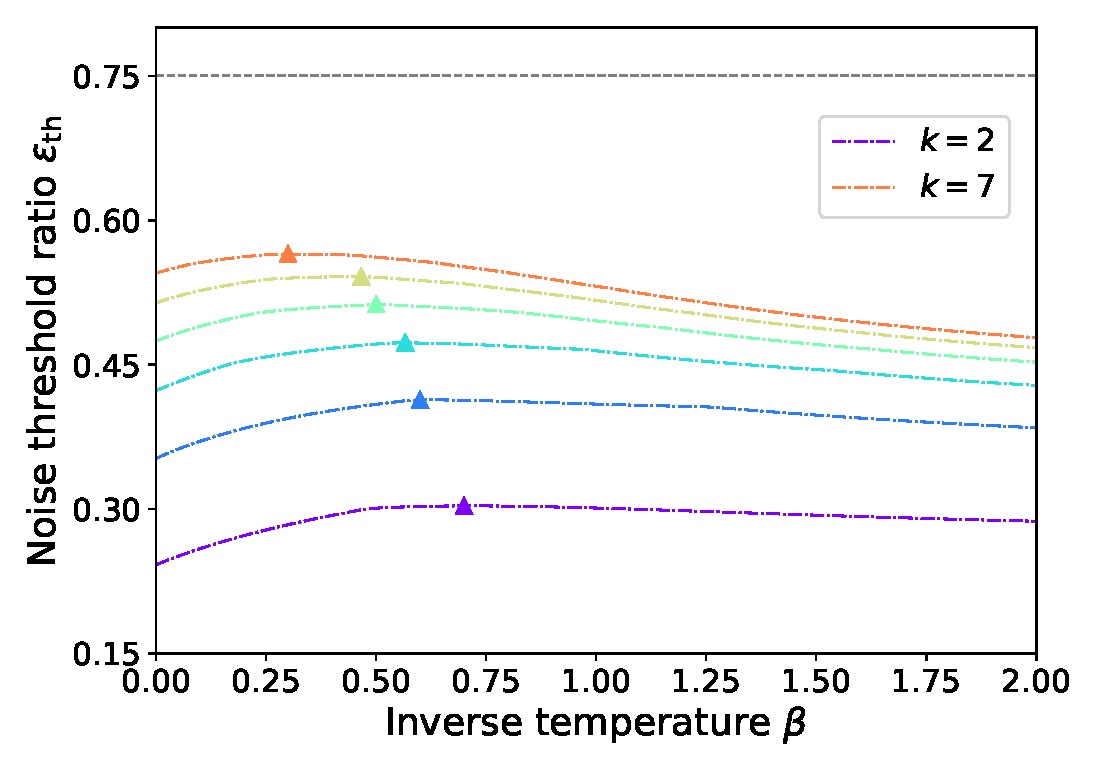
\includegraphics[scale=0.5]{figs/thermal_distill.pdf}
    \caption{\textbf{Threshold dependence on temperature in thermal fragments.} Lorenz curve ratios for the Strange state purifying process in~\cref{eq:sdist} with $\epsilon' = 0.05$.
    The peaks of each curve indicate the optimal temperature $\beta_{\rm{max}}^{-1}$ that allows for the highest noise threshold at every given number of initial state copies $k$.
    The line $\epsilon = \frac{3}{4}$ indicates the threshold noise beyond which the Strange state no longer contains negativities.
    }
    \label{fig:thermal_distill}
\end{figure}










































































\end{document}